\documentclass[border=4pt]{standalone}
\usepackage{amsmath,amssymb,tikz}\usetikzlibrary{arrows.meta}
\definecolor{figB}{RGB}{31,90,166}\definecolor{figR}{RGB}{176,48,48}\definecolor{figG}{RGB}{46,125,50}\definecolor{figO}{RGB}{214,120,20}
% Left: q = 3x^2+2xy+3y^2 = 4u^2+2w^2, u along (1,1)/sqrt2, w along (-1,1)/sqrt2; level sets q = 1,2,3
% (semi-axes sqrt(c)/2 along u, sqrt(c/2) along w). Right: q = 2xy = u^2 - w^2, levels 2xy = +-0.5, +-1.5.
\begin{document}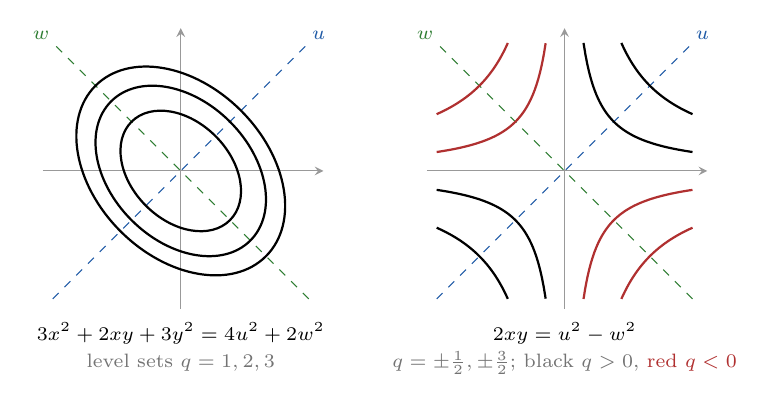
\begin{tikzpicture}[scale=1.25,>={Stealth[length=1.8mm]}]
\begin{scope}
\draw[black!40,thin,-stealth] (-1.4,0)--(1.45,0); \draw[black!40,thin,-stealth] (0,-1.4)--(0,1.45);
\draw[dashed,figB] (-1.3,-1.3)--(1.3,1.3) node[above right,font=\scriptsize,inner sep=1pt]{$u$};
\draw[dashed,figG] (1.3,-1.3)--(-1.3,1.3) node[above left,font=\scriptsize,inner sep=1pt]{$w$};
\foreach \c in {1,2,3} { \draw[thick,rotate=45] (0,0) ellipse ({sqrt(\c)/2} and {sqrt(\c)/sqrt(2)}); }
\node[font=\scriptsize] at (0,-1.65) {$3x^2+2xy+3y^2=4u^2+2w^2$};
\node[font=\scriptsize,black!55] at (0,-1.95) {level sets $q=1,2,3$};
\end{scope}
\begin{scope}[xshift=3.9cm]
\draw[black!40,thin,-stealth] (-1.4,0)--(1.45,0); \draw[black!40,thin,-stealth] (0,-1.4)--(0,1.45);
\draw[dashed,figB] (-1.3,-1.3)--(1.3,1.3) node[above right,font=\scriptsize,inner sep=1pt]{$u$};
\draw[dashed,figG] (1.3,-1.3)--(-1.3,1.3) node[above left,font=\scriptsize,inner sep=1pt]{$w$};
\foreach \c in {0.25,0.75} {
 \draw[thick,domain={\c/1.3}:1.3,samples=60] plot (\x,{\c/\x}); \draw[thick,domain={-1.3}:{-\c/1.3},samples=60] plot (\x,{\c/\x});
 \draw[thick,figR,domain={\c/1.3}:1.3,samples=60] plot (\x,{-\c/\x}); \draw[thick,figR,domain={-1.3}:{-\c/1.3},samples=60] plot (\x,{-\c/\x}); }
\node[font=\scriptsize] at (0,-1.65) {$2xy=u^2-w^2$};
\node[font=\scriptsize,black!55] at (0,-1.95) {$q=\pm\tfrac12,\pm\tfrac32$; black $q>0$, \textcolor{figR}{red $q<0$}};
\end{scope}
\end{tikzpicture}\end{document}
